% !TEX root = ../thesis.tex

\chapter{二维Markov跳变系统的异步二次型控制}
	二次型控制也是一种典型的控制方法,近年来,Markov跳变系统的二次型控制问题也得到了广泛的研究并取得了一系列的重要成果\cite{ji1990controllability,costa1999constrained,do2016quadratic}。文献\cite{zabala2019detector}对模态不匹配的1D-Markov跳变系统二次型进行了讨论,探究了不同初始条件的最优成本性能。文献\cite{guan2001robust,dhawan2007optimal,dhawan2010lmi}对2D系统下的Rosser模型和FM模型的保成本控制进行了讨论,并在文献中对初始状态做出了一些基本假设。
	
	本章中,我们将探究基于Rosser模型的2D-Markov跳变系统的二次型控制问题。考虑控制模态同系统模态的不匹配问题,我们引入隐Markov模型设计了一个线性状态反馈控制器。根据2D系统的结构和特性定义了一个成本函数,并根据初始条件的不同情况分别对系统的最优成本性能展开讨论。

\section{数学模型及问题描述}
	本章考虑如下Roesser模型下的二维Markov跳变系统
	\begin{equation} \label{qc-system-equation}
	\left\{
	\begin{array}{lr}
	\hat{x}(i,j) = A_{r(i,j)}x(i,j)+B_{r(i,j)}u(i,j) \\
	z(i,j) = C_{r(i,j)}x(i,j)+D_{r(i,j)}u(i,j)
	\end{array}
	\right.
	\end{equation}
	其中,
	\begin{equation*}
	\hat{x}(i,j) = \begin{bmatrix}
	x^{h}(i+1,j) \\
	x^{v}(i,j+1)
	\end{bmatrix}, \
	x(i, j) = \begin{bmatrix}
	x^{h}(i,j) \\
	x^{v}(i,j)
	\end{bmatrix},
	\end{equation*}
	这里$x^{h}(i,j)\in\mathbb{R}^{n_1}$,$x^{v}(i,j)\in\mathbb{R}^{n_2}$分别表示水平、垂直方向的系统子状态,$u(i,j)\in\mathbb{R}^{m}$表示系统控制输入,$z(i,j)\in\mathbb{R}^{l}$表示系统被控输出。$A_{r(i,j)}$,$B_{r(i,j)}$,$C_{r(i,j)}$及$D_{r(i,j)}$是具有合适维度的已知系统时变矩阵,并且是$r(i,j)$的函数。$r(i,j)$表示一个随机跳变过程,可以用来表示Markov链,在集合$\mathcal{N}_{1} = \{1,2...N_{1}\}$中取值,并且满足具有如下状态转移概率的状态转移矩阵$\varLambda = \{\lambda_{kp}\}$
	\begin{equation}\label{qc-tps-system}
	\begin{split}
	&\Pr\{r(i+1,j)=p|r(i,j)=k\}\\
	=&\Pr\{r(i,j+1)=p|r(i,j)=k\}=\lambda_{kp},\  \forall k,p \in \mathcal{N}_{1}
	\end{split}
	\end{equation}
	且对任意的$k, p\in\mathcal{N}_{1}$,$\lambda_{kp}$ 满足
	\begin{equation}
	\left\{
	\begin{array}{lr}
	\lambda_{kp} \geq 0, \\
	\sum_{p=1}^{N_1}\lambda_{kp}=1.
	\end{array}
	\right.
	\end{equation}
	
	在实际应用系统中,由于控制器不能完全的获得系统的模态信息,因此,在本章中,我们基于隐Markov模型,设计如下异步控制器
	\begin{equation}\label{qc-controller}
	u(i,j) = K_{\sigma(i,j)}x(i,j),
	\end{equation}
	其中$K_{\sigma(i,j)}\in \mathbb{R}^{(n_1+n_2)\times m}$是待决定的控制器增益矩阵,$\sigma(i,j)$表示控制器模态,在集合$\mathcal{N}_{2} = \{1,2...N_{2}\}$中取值,并且满足具有如下条件状态转移概率的状态转移矩阵 $\varPsi=\{\mu_{k\tau }\}$
	\begin{equation}
	\Pr\{\sigma(i,j)=s|r(i,j)=k\}=\mu_{ks }, %\forall  k\in\mathcal{N}_{1}, \tau\in\mathcal{N}_{2},
	\end{equation}
	且,对任意的$k\in\mathcal{N}_{1}, s\in\mathcal{N}_{2}$,有 $\mu_{k\tau }\in[0,1]$,对任意的$k$,有  $\sum_{s =1}^{N_{2}}\mu_{ks } = 1$。
	
	然后,在本章中,我们对初始条件($X_{0},\varGamma_{0}$)定义如下:
	\begin{equation*}
		\left\{
			\begin{array}{lr}
				X_{0}\equiv \big\{x^{h}(0,0),x^{h}(0,1),x^{h}(0,2),\cdots, x^{v}(0,0),x^{v}(1,0),x^{v}(2,0),\cdots  \big\},\\
				\varGamma_{0}\equiv \big\{r(0,0), r(0,1),r(0,2),\cdots,r(1,0),r(2,0),\cdots \big\}.
			\end{array}
		\right.
	\end{equation*}
	
	下面,我们对初始状态$X_{0}$做下面几个假设:
	
	{\bf 假设 \ \ 4.1:}
	2D系统\eqref{qc-system-equation}的零初始状态为,对任意的非负整数$i,j$,有$x^{h}(0,j) =0, x^{v}(i,0)=0$。
	
	{\bf 假设 \ \ 4.2:}
	系统\eqref{qc-system-equation}的初始状态$X_{0}$满足
	\begin{equation}
	\mathscr{X}_{0} \equiv \lim\limits_{L\to\infty}\mathbb{E}\Big\{\sum_{l=1}^{L}(\|x^{h}(0,l)\|^{2}+ \|x^{v}(l,0)\|^{2})\Big\} < \infty
	\end{equation}
	这里 $\mathbb{E}\{\cdot\}$ 表示数学期望,且,我们称系统的全部初始状态之和是有界的。
	
	{\bf 假设 \ \ 4.3:}
	在假设4.2的基础上,我们进一步假设,存在两个正整数$l_1$,$l_2$,使得
	\begin{equation}
		\left\{
		\begin{array}{lr}
		x^{h}(0,j)=0,\quad j\geq l_1,\\
		x^{v}(i,0)=0,\quad i\geq l_2.
		\end{array}
		\right.
	\end{equation}
	此时,系统只有有限个非零初始状态。
	
	{\bf 假设 \ \ 4.4:}
	在假设4.3的基础上,我们进一步做如下假设。存在$L(0,j)$,$L(i,0)$,$Z_1$,$Z_2$,使得对任意的$j<l_1,i<l_2$有
	\begin{equation}
		\left\{
		\begin{array}{lr}
		x^{h}(0,j)=Z_1L(0,j),\quad L^{T}(0,j)L(0,j)\leq 1,\\
		x^{v}(i,0)=Z_2L(i,0),\quad  L^{T}(i,0)L(i,0)\leq 1.
		\end{array}
		\right.
	\end{equation}
	此时,我们称系统的只有有限个非零初始状态,且每一个非零初始状态都是有界的。
	
	{\bf 注 \ \ 4.1:}
	实际上,不难发现,对于任意给定的$x^{h}(0,j)$,$x^{v}(i,0)$,我们总是可以通过选择合适的$Z_1$,$Z_2$及$L(0,j)$,$L(i,0)$对其进行表示。这个初始条件的假设思路已经在文献[123]中使用了,不过,值得注意的是,在上述文献中,都假设水平、垂直状态的初始状态是分别一样的,而在我们的假设中,并没有这么强的约束,因此更加贴近实际情况。
	
	下面,我们给出系统\eqref{qc-system-equation}的稳定性及成本函数的定义
	
	{\bf 定义 \ \ 4.1:}
	如果下式对任意的初始条件$X_{0}$成立
	\begin{equation}\label{qc-AMSS}
	\lim\limits_{i+j\to\infty}\mathbb{E}\{\|x(i,j)\|^{2}\} = 0
	\end{equation}
	我们称,在假设4.1意义下的系统\eqref{qc-system-equation}是渐进均方稳定的。
	
	本章中,我们考虑如下成本函数
	\begin{equation}\label{qccostfuntion}
	\begin{split}
	J(i,j) \equiv \|z\|_{2}^{2} = \sum_{i=0}^{\infty}\sum_{j=0}^{\infty}E(\|z(i,j)\|^{2})\\
	\end{split}
	\end{equation}
	
	由系统\eqref{qc-system-equation}及控制器\eqref{qc-controller}可以得到闭环2D控制系统的方程为
	\begin{equation}\label{qc-closed-system-equation}
		\left\{
			\begin{array}{lr}
				\hat{x}(i,j) = (A_{r(i,j)}+B_{r(i,j)}K_{\sigma(i,j)})x(i,j), \\
				z(i,j) = (C_{r(i,j)}+D_{r(i,j)}K_{\sigma(i,j)})x(i,j).
			\end{array}
		\right.
	\end{equation}
	
	本章的目标为,设计异步控制器$K_{\sigma(i,j)}$,使得闭环控制系统渐进均方稳定,且满足一定的保成本性能$J^{*}$,针对初始条件的不同,我们分为下面三种情况进行讨论
	
	(1) 初始状态$X_{0}$已知(假设4.3成立),且初始模态$\varGamma_{0}$已知。
	
	(2) 初始状态$X_{0}$未知,但满足假设4.4,且初始模态$\varGamma_{0}$已知。
	
	(3) 初始状态$X_{0}$未知,但满足假设4.4,且初始模态$\varGamma_{0}$未知。
	

\section{主要结论}
	在本节,我们首先探究闭环控制系统\eqref{qc-closed-system-equation}的稳定性问题,然后,针对初始条件$(X_{0}, \varGamma_{0})$的三种不同情况,分别讨论他们的保成本性能。
	
	{\bf 定理 \ \ 4.1:} 
	考虑闭环控制系统\eqref{qc-closed-system-equation},当系统初始状态满足假设4.3,且系统初始模态已知时候,若对任意的$k\in\mathcal{N}_{1}$,$s\in\mathcal{N}_2$,存在正定矩阵$R_{k}=\mathrm{diag}\{R^{h}_{k},R^{v}_{k}\}$,$Q_{ks}$,矩阵$K_{s}$,使得下列不等式成立,
	\begin{equation}\label{qc-T1-1}
	\sum_{s=1}^{N_2}u_{ks}Q_{ks}-R_{k}< 0,
	\end{equation}
	\begin{equation}\label{qc-T1-2}
	\bar{A}^{T}_{ks}\mathcal{R}_{k}\bar{A}_{ks}+\bar{C}^{T}_{ks}\bar{C}_{ks}-Q_{ks}<0,
	\end{equation}
	其中,$\bar{A}_{ks}=A_{k}+B_kK_s$,$\bar{C}_{ks}=C_k+D_kK_s$,$\mathcal{R}_{k}=\sum_{s =1}^{N_1}\lambda_{kp}R_p$。则,系统是渐进均方稳定的,且,相对应的保成本性能为
	\begin{equation}\label{qcT1C3}
		J(i,j)\leq  \sum_{j=0}^{l_1-1}V_{1}(0,j)+\sum_{i=0}^{l_2-1}V_2(i,0).
	\end{equation}
	其中,$V_{1}(i,j)$ 及 $V_{2}(i,j)$ 定义如下  
	\begin{equation*}
	\left\{
	\begin{array}{lr}
	\begin{split}
	V_{1}(i,j)=x^{hT}(i,j)R^{h}_{r(i,j)}x^{h}(i,j),\\
	V_{2}(i,j)=x^{vT}(i,j)R^{v}_{r(i,j)}x^{v}(i,j).
	\end{split}
	\end{array}
	\right.
	\end{equation*}
	{\bf 证明:} 
	首先,我们选择如下李雅普诺夫函数,
	\begin{equation*}
		V(i,j) = x^{T}(i,j)R_{r(i,j)}x(i,j)
	\end{equation*}
	令
	\begin{equation*}
	\hat{V}(i,j) = \hat{x}^{T}(i,j)\mathrm{diag}\{R^{h}_{r(i+1,j)},R^{v}_{r(i,j+1)}\}\hat{x}(i,j)
	\end{equation*}
	那么,由闭环控制系统\eqref{qc-closed-system-equation}和转移概率函数\eqref{qc-tps-system},我们可以推出
	\begin{equation}\label{qc-diff1}
		\begin{split}
			\mathbb{E}\{\varDelta V(i,j)\}&=\mathbb{E}\{\hat{V}(i,j)-V(i,j) \}\\
				&=\mathbb{E}\{\hat{x}^{T}(i,j)\mathcal{R}_{k}\hat{x}(i,j) \}- x^{T}(i,j)R_{k}x(i,j)\\
				&= x^{T}(i,j)\{\sum_{s=1}^{N_2}u_{ks} \bar{A}^{T}_{ks}\mathcal{R}_{k}\bar{A}_{ks} -R_{k} \}x(i,j)  
		\end{split}
	\end{equation}
	由\eqref{qc-T1-1}-\eqref{qc-T1-2},我们可以得到
	\begin{equation}\label{qc-dif1}
		\sum_{s =1}^{N_2}u_{ks}\bar{A}^{T}_{ks}\mathcal{R}_{k}\bar{A}_{ks}-R_{k}<0
	\end{equation}
	因此,由\eqref{qc-diff1}-\eqref{qc-dif1},我们可以进一步推出
	\begin{equation}\label{qc18}
		\mathbb{E}\{\varDelta V(i,j)\} < -\alpha \mathbb{E}\{\|x(i,j)\|^{2} \}
	\end{equation}
	这里,$\alpha$表示$(R_{k}-\sum_{s =1}^{N_2}u_{ks}\bar{A}^{T}_{ks}\mathcal{R}_{k}\bar{A}_{ks})$的最小特征值。显然,$\alpha$是一个正数。对\eqref{qc18}两边做累加,我们可以推出
	\begin{equation}
		\mathbb{E}\{ \sum_{i=0}^{l_2-1}\sum_{j=0}^{l_1-1}\|x(i,j)\|^{2} \}<-\frac{1}{\alpha}\mathbb{E}\{\sum_{i=0}^{l_2-1}\sum_{j=0}^{l_1-1}\varDelta V(i,j) \}
	\end{equation}
	这里,$l_1$,$l_2$已经定义在假设4.3中。接下来,我们使用$R_{k}=\mathrm{diag}\{R^{h}_{k},R^{v}_{k}\}$,$\mathbb{E}\{\varDelta V(i,j)\}=\mathbb{E}\{\hat{V}(i,j)-V(i,j) \}$,将水平,垂直状态分开,可以推出
	\begin{equation} \label{qc19}
	\begin{split}
	&\sum_{i=0}^{l_2-1}\sum_{j=0}^{l_1-1}  \varDelta V(i,j)\\&= \sum_{i=0}^{l_2-1}\big\{V_2(i,l_1) - V_2(i,0) \big\}+  \sum_{j=0}^{l_1-1}\big\{V_1(l_2,j) - V_1(0,j) \big\}\\
	&\leq -\big( \sum_{i=0}^{l_2-1}V_2(i,0) + \sum_{j=0}^{l_1-1}V_{1}(0,j)\big) \\
	%			&\leq -\beta \sum_{\ell=0}^{\infty} \big(  \|x^{v}(\ell,0)\|^{2} + \|x^{h}(0,\ell)\|^{2} \big)
	\end{split}
	\end{equation} 
	由\eqref{qc18}-\eqref{qc19}可以推出
	\begin{equation}\label{qc20}
	\begin{split}
	\mathbb{E}\Big\{\sum_{i=0}^{\infty}\sum_{j=0}^{\infty}  \|x(i,j)\|^{2} \Big\} &\leq \frac{\beta}{\alpha} \sum_{\ell=0}^{\infty} \big(  \|x^{v}(\ell,0)\|^{2} + \|x^{h}(0,\ell)\|^{2} \big)<\infty
	\end{split}	
	\end{equation}
	这里的$\beta$是$R^{h}_{r(i,j)}$,$R^{v}_{r(i,j)}$的最大特征值。显然,上式可以保证\eqref{qc-AMSS}成立,因此,研究的系统是渐进均方稳定的。
	现在,我们对成本性能进行分析,由\eqref{qc-T1-1}-\eqref{qc-T1-2},可以推出
	\begin{equation}
		\begin{split}
			\mathbb{E}\{\|z(i,j)\|^{2}+\varDelta V(i,j) \}=x^{T}(i,j)\{\sum_{s=1}^{N_2}u_{ks} \bar{A}^{T}_{ks}\mathcal{R}_{k}\bar{A}_{ks} +C^{T}_{ks}C_{ks}-R_{k} \}x(i,j)<0
		\end{split}
	\end{equation}
	对上式做累加得到
	\begin{equation}
	\begin{split}
	&\sum_{i=0}^{\infty}\sum_{j=0}^{\infty}\mathbb{E}\{\|z(i,j)\|^{2}+\varDelta V(i,j) \}\\&=J(i,j)+\sum_{i=0}^{\infty}\sum_{j=0}^{\infty}\mathbb{E}\{\varDelta V(i,j) \}\\
	&<J(i,j)-\big( \sum_{i=0}^{l_2-1}V_2(i,0) + \sum_{j=0}^{l_1-1}V_{1}(0,j)\big)\\&<0
	\end{split}
	\end{equation}
	因此,
	\begin{equation}
		J(i,j)<\big( \sum_{i=0}^{l_2-1}V_2(i,0) + \sum_{j=0}^{l_1-1}V_{1}(0,j)\big)
	\end{equation}
	至此,定理证明结束。
	
	{\bf 注 \ \ 4.2:}
	仔细检查定理4.1的推导,我们不难发现,其实,假设4.2即可以保证闭环控制系统的稳定性。


	{\bf 定理 \ \ 4.2:}
	考虑闭环控制系统\eqref{qc-closed-system-equation},当系统初始状态满足假设4.4,初始模态已知时,若对任意的$k\in\mathcal{N}_{1}$,$s\in\mathcal{N}_2$,存在正定矩阵$R_{k}=\mathrm{diag}\{R^{h}_{k},R^{v}_{k}\}$,$Q_{ks}$,矩阵$K_{s}$,使得不等式\eqref{qc-T1-1}-\eqref{qc-T1-2}成立,则,系统是渐进均方稳定的,且,相对应的保成本性能为
	\begin{equation}\label{qcT2}
	\begin{split}
	J(i,j) \leq \sum_{\varrho_{1}=1}^{N_{1}}\varpi_{\varrho_{1}}\lambda_{max}(Z^{T}_{1}R^{h}_{\varrho_{1}}Z_{1})
	+\sum_{\varrho_{2}=1}^{N_{1}}\omega_{\varrho_{2}}\lambda_{max}(Z^{T}_{2}R^{v}_{\varrho_{2}}Z_{2})
	\end{split}
	\end{equation}
	这里,$\varrho_{1}$,$\varrho_{2}$分别表示系统、控制器的模态,$\varpi_{\varrho_{1}}$,$\omega_{\varrho_{2}}$分别表示初始模态中,对应的系统模态等于$\varrho_{1}$,控制器模态等于$\varrho_{2}$的数量。
	
	{\bf 证明:} 
	我们选择跟定理4.1一样的李雅普诺夫函数,稳定性不难发现已经可以由\eqref{qc-T1-1}-\eqref{qc-T1-2}保证。同时,由于假设4.4是在假设4.3基础上的进一步加强,那么不难推出,当系统满足假设4.4时,可以保证\eqref{qcT1C3}成立。由假设4.4,我们同时可以推出
	\begin{equation}
		\begin{split}
			J(i,j)&\leq \varpi_1\lambda_{max}(Z^{T}_{1}R^{h}_{1}Z_{1})+\dots+\varpi_{N_{1}}\lambda_{max}(Z^{T}_{1}R^{h}_{N_{1}}Z_{1}) \\ 
			&+\omega_{1}\lambda_{max}(Z^{T}_{2}R^{v}_{1}Z_{2})+\dots+\omega_{N_{2}}\lambda_{max}(Z^{T}_{2}R^{v}_{N_2}Z_{2})\\
			&=\sum_{\varrho_{1}=1}^{N_{1}}\varpi_{\varrho_{1}}\lambda_{max}(Z^{T}_{1}R^{h}_{\varrho_{1}}Z_{1})
			+\sum_{\varrho_{2}=1}^{N_{1}}\omega_{\varrho_{2}}\lambda_{max}(Z^{T}_{2}R^{v}_{\varrho_{2}}Z_{2})
		\end{split}
	\end{equation}
	至此,证明完毕。
	
	{\bf 定理 \ \ 4.3:}
	考虑闭环控制系统\eqref{qc-closed-system-equation},当系统初始状态满足假设4.4,初始模态未知时,若对任意的$k\in\mathcal{N}_{1}$,$s\in\mathcal{N}_2$,存在正定矩阵$\bar{R}_{k}=\mathrm{diag}\{\bar{R}^{h}_{k},\bar{R}^{v}_{k}\}$,$\bar{Q}_{ks}$,矩阵$\bar{K}_{s}$,$T_{s}$,使得下列不等式成立
	\begin{equation}\label{qcT3C1}
	\begin{bmatrix}
	-\lambda_1I &Z^{T}_1\\
	*&-\bar{R}^{h}_{k}
	\end{bmatrix}<0
	\end{equation}
	\begin{equation}\label{qcT3C2}
	\begin{bmatrix}
	-\lambda_2I &Z^{T}_{2}\\
	*&-\bar{R}^{v}_{k}
	\end{bmatrix}<0
	\end{equation}
	\begin{equation}\label{qcT3C3}
	\begin{bmatrix}
	-\bar{R}_{k}& \sqrt{u_{k1}}\bar{R}_{k} &\cdots&\sqrt{u_{kN_2}}\bar{R}_{k}\\
	*&-\bar{Q}_{k1}&\cdots&0\\
	*&*&\ddots&0\\
	*&*&*&-\bar{Q}_{kN_2}\\
	\end{bmatrix}<0
	\end{equation}
	\begin{equation}\label{qcT3C4}
	\begin{bmatrix}
		\bar{Q}_{ps}-T_{s}-T^{T}_{s} & C_{k}T_s+D_k\bar{K}_s& \sqrt{\lambda_{k1}}(A_kT_s+B_k\bar{K}_s)&\cdots&\sqrt{\lambda_{kN_1}}(A_kT_s+B_k\bar{K}_s)\\
				*&-I&0&\cdots&0\\
				*&*&-\bar{R}_1&\cdots&0\\
				\vdots&\vdots&\vdots&\ddots&0\\
				*&*&*&*&-\bar{R}_{N_1}\\
				
	\end{bmatrix}<0
	\end{equation}	
	则,系统是渐进均方稳定的,且对应的保成本性能为
	\begin{equation}
	\begin{split}
	J(i,j) \leq l_1\lambda_1 + l_2\lambda_2
	\end{split}
	\end{equation}
	{\bf 证明:} 定义$\bar{R}_{k}=R^{-1}_{k}$,$\bar{Q}_{ks}=Q^{-1}_{ks}$,$\bar{K}_s=K^{-1}_s$。
	对\eqref{qcT3C3}两边同时灯以$\mathrm{diag}\{R^{k},I,\dots,I \}$,可以得到
	\begin{equation} 
	\begin{bmatrix}
	-R_{k}& \sqrt{u_{k1}}R_{k} &\cdots&\sqrt{u_{kN_2}}R_{k}\\
	*&-\bar{Q}_{k1}&\cdots&0\\
	*&*&\ddots&0\\
	*&*&*&-\bar{Q}_{kN_2}\\
	\end{bmatrix}<0
	\end{equation}
	然后,根据Schur补引理,可以得到\eqref{qc-T1-1}成立。
	不难发现\eqref{qcT3C4}可以推出下式
	\begin{equation} 
	\begin{bmatrix}
	T^{T}_{s}\bar{Q}_{ps}T_{s} & C_{k}T_s+D_k\bar{K}_s& \sqrt{\lambda_{k1}}(A_kT_s+B_k\bar{K}_s)&\cdots&\sqrt{\lambda_{kN_1}}(A_kT_s+B_k\bar{K}_s)\\
	*&-I&0&\cdots&0\\
	*&*&-\bar{R}_1&\cdots&0\\
	\vdots&\vdots&\vdots&\ddots&0\\
	*&*&*&*&-\bar{R}_{N_1}\\
	\end{bmatrix}<0
	\end{equation}
	使用$\mathrm{diag}\{T^{-1}_s,I,\dots,I \}$及其转置分别左乘,右乘上式,然后再使用Schur补引理,可以推出\eqref{qc-T1-2}成立。
	这样,系统的稳定性可以保证。
	根据假设4.3,由于系统的初始模态并不知道,我们无法确定系统每个模态对应的数量。因此,我们需要对任意的系统模态下,$\lambda_{max}(Z^{T}_{1}R^{h}_{\varrho_{1}}Z_{1})$,$\lambda_{max}(Z^{T}_{2}R^{v}_{\varrho_{2}}Z_{2})$分别得到确定一个统一的上界。
	由\eqref{qcT3C1}-\eqref{qcT3C2}可以得到
	\begin{equation}
		\begin{split}
			&Z^{T}_1R^{h}_{k}Z_1<\lambda_1I,\\ &Z^{T}_2R^{v}_{k}Z_2<\lambda_2I	
		\end{split}
	\end{equation}
	这里,$\lambda_1$是对全部系统模态,$\lambda_{max}(Z^{T}_{1}R^{h}_{\varrho_{1}}Z_{1})$的上界,$\lambda_2$是对全部系统模态,$\lambda_{max}(Z^{T}_{2}R^{v}_{\varrho_{2}}Z_{2})$的上界。
	因此,由\eqref{qcT2}可以推出
	\begin{equation}
		J(i,j) \leq l_1\lambda_1 + l_2\lambda_2
	\end{equation}
	至此,定理证明完毕。
	
	{\bf 注 \ \ 4.2:}
	本章中,可以先通过下面的最优化问题求解出$\bar{K}_s$
	\begin{equation}\label{qc_optimization-problem}
	\text{min $(l_1\lambda_1 + l_2\lambda_2)$ subject to \eqref{qcT3C1}-\eqref{qcT3C4}}。
	\end{equation}
	然后通过$K_s=\bar{K}_sT^{-1}_s$来求解出异步控制器增益。

\section{数值例子}
	在本节,我们将选择一个简单的数值仿真例子,来验证设计的异步二次型控制器的有效性。首先,我们选择控制器模态、系统模态都为2,即$N_1=N_2=2$。然后选择系统参数如下
	
	模态一:
	\begin{equation} \notag
	\begin{aligned}
	A_{1} &= \begin{bmatrix}
	-1.0&0.6\\
	-0.2&-1.3
	\end{bmatrix}, \ 
	B_{1} = \begin{bmatrix}
	0.2&0.1\\ 1.2&0.8
	\end{bmatrix} ,\
		C_{1} &= \begin{bmatrix}
	1&0\\1.2&0.8
	\end{bmatrix},\
	D_{1} = \begin{bmatrix}
	-0.1&0\\0&0.1
	\end{bmatrix}
	\end{aligned}  
	\end{equation}
	
	模态二:
	\begin{equation} \notag
	\begin{aligned}
	A_{2} &= \begin{bmatrix}
	-1.2&0.6\\
	-0.4&-1.2
	\end{bmatrix}, \ 
	B_{2} = \begin{bmatrix}
	0.3&0.2\\ 1.0&0.8
	\end{bmatrix} ,\
	C_{2} &= \begin{bmatrix}
	1.2&0\\1.0&0.8
	\end{bmatrix},\
	D_{2} = \begin{bmatrix}
	-0.1&0\\0&0.1
	\end{bmatrix}
	\end{aligned}  
	\end{equation}
	
	系统的模态转移矩阵$\varPi$、控制器的条件模态转移矩阵$\varPsi$分别设置为
	\begin{equation}
		\varPi = \begin{bmatrix}
		0.8& 0.2\\ 0.3& 0.7
		\end{bmatrix},    %system mode transfer function.
		\varPsi = \begin{bmatrix}
			0.6& 0.4\\0.4 &0.6
		\end{bmatrix}
	\end{equation}
	
	
	初始状态我们设置为:
	\begin{equation*}
	\begin{aligned}
	x^{h}(0, j)&=\begin{cases}
	0.1, \quad 0\leq j \leq 10 \\
	0, \quad \ \ elsewhere
	\end{cases} \\
	x^{v}(i, 0)&=\begin{cases}
	0.1, \quad 0\leq i \leq 10 \\
	0, \quad \ \ elsewhere
	\end{cases}
	\end{aligned}
	\end{equation*}
	
	根据假设4.4,我们不难发现,对任意的$i\leq10,j\leq10$,可以选择$L(i,0)=L(0,j)=1$,相应的$Z_1=Z_2=0.1$。
	
	当没有施加异步控制器时,系统在水平方向、垂直方向的状态轨迹分别绘制于图\ref{figqchstate}、图\ref{figqcvstate}中。不难发现,当$u(i,j)=0$,即不施加控制反馈作用时,系统水平方向、垂直方向的状态轨迹都是离散的,表明,此时系统不稳定。
	
	\begin{figure}[!htb]
		\centering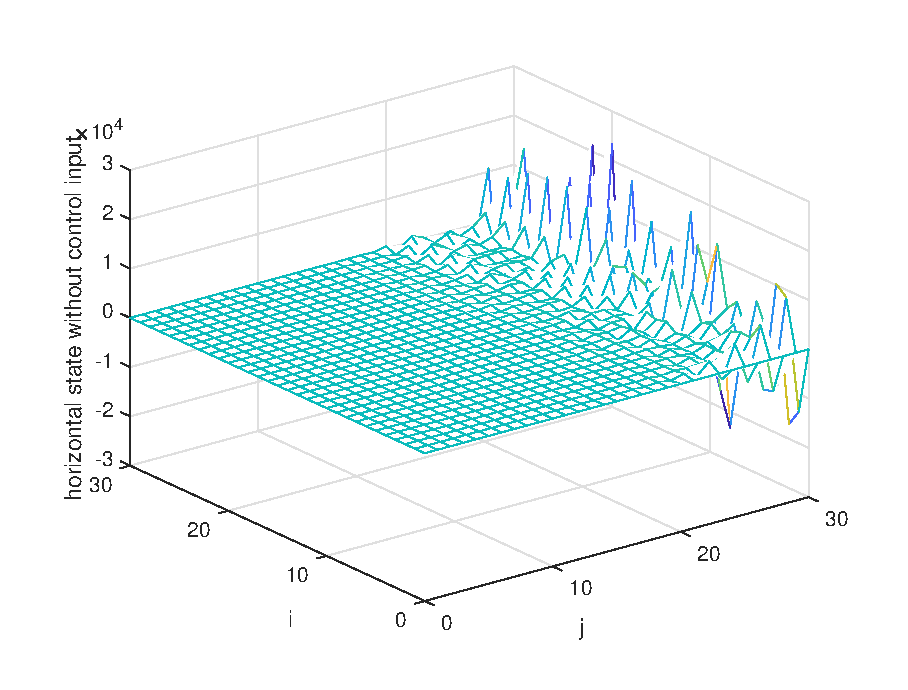
\includegraphics[scale=0.6]{./figures/qc/simulation/hstateU0.eps}\\ 
		\caption{$u(i,j)=0$时的水平状态 $x^{h}(i,j)$}
		\label{figqchstate}
	\end{figure}
	
	\begin{figure}[!htb]
		\centering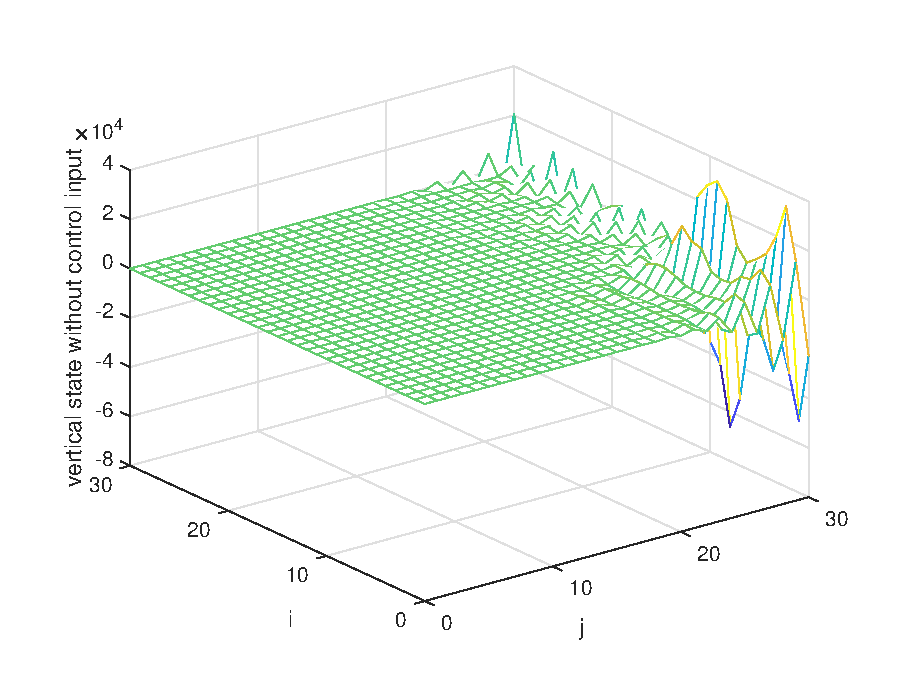
\includegraphics[scale=0.6]{./figures/qc/simulation/vstateU0.eps}\\ 
		\caption{$u(i,j)=0$时的垂直状态 $x^{v}(i,j)$}
		\label{figqcvstate}
	\end{figure}
	
	下面我们通过求解最优化问题\eqref{qc_optimization-problem},可以得到如下控制器矩阵增益
	
	模态一:
	\begin{equation*}
	K_{1}=\begin{bmatrix}
	 6.1883   &-2.0444\\
	-5.5118   &-3.4863
	\end{bmatrix}
	\end{equation*}
	
	模态二:
	\begin{equation*}
	K_{2} = 	\begin{bmatrix}
	6.5645   &-0.8006\\
	-5.5108   &-4.2340
	\end{bmatrix}
	\end{equation*}
	
	同时,系统的最小保成本性能$J^{*}=0.4512$。然后,施加了控制器以后的系统水平、垂直状态轨迹分别绘制于图\ref{figqchstate1}、图\ref{figqcvstate1}中。显然,当施加了异步二次型控制器以后,系统在水平、垂直方向的状态轨迹都收敛了,表明,此时系统是稳定的。同时,控制作用$u(i,j)$在水平方向、垂直方向的作用效果分别绘制于图\ref{figqcuh}、图\ref{figqcuv}中。综合仿真结果,可以得出结论,本章中设计的控制器是有效的。
	\begin{figure}[!htb]
		\centering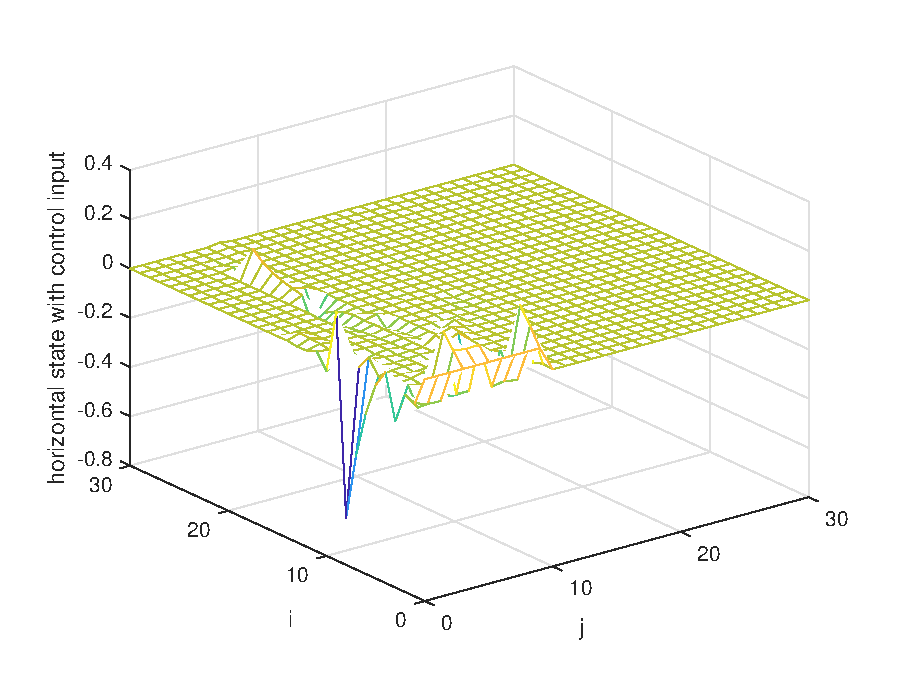
\includegraphics[scale=0.6]{./figures/qc/simulation/hstate.eps}\\ 
		\caption{异步二次型控制下的水平状态 $x^{h}(i,j)$}
		\label{figqchstate1}
	\end{figure}
	
	\begin{figure}[!htb]
		\centering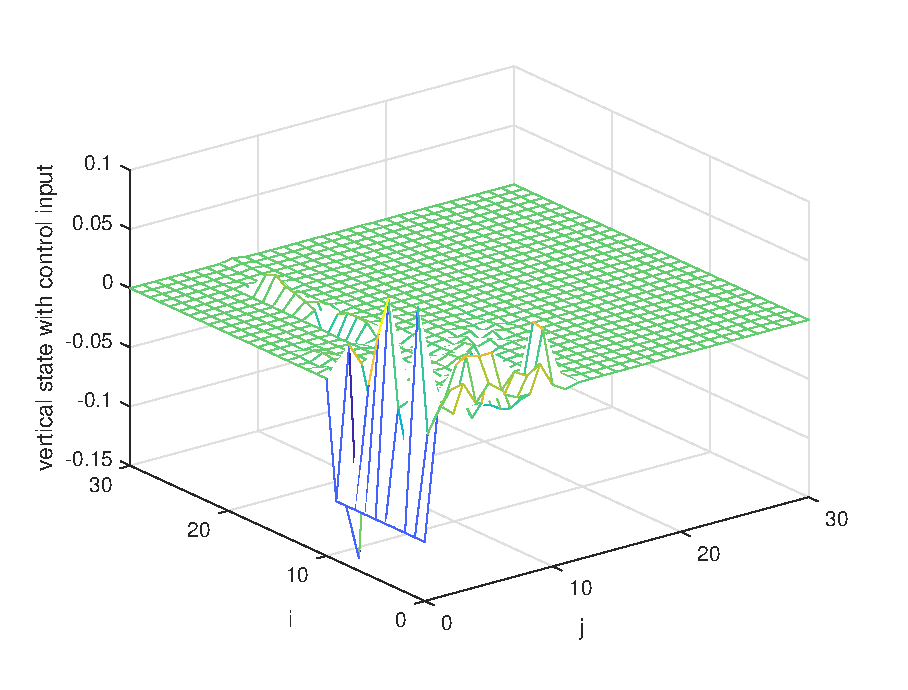
\includegraphics[scale=0.6]{./figures/qc/simulation/vstate.eps}\\ 
		\caption{异步二次型控制下的垂直状态 $x^{v}(i,j)$}
		\label{figqcvstate1}
	\end{figure}
	
	\begin{figure}[!htb]
		\centering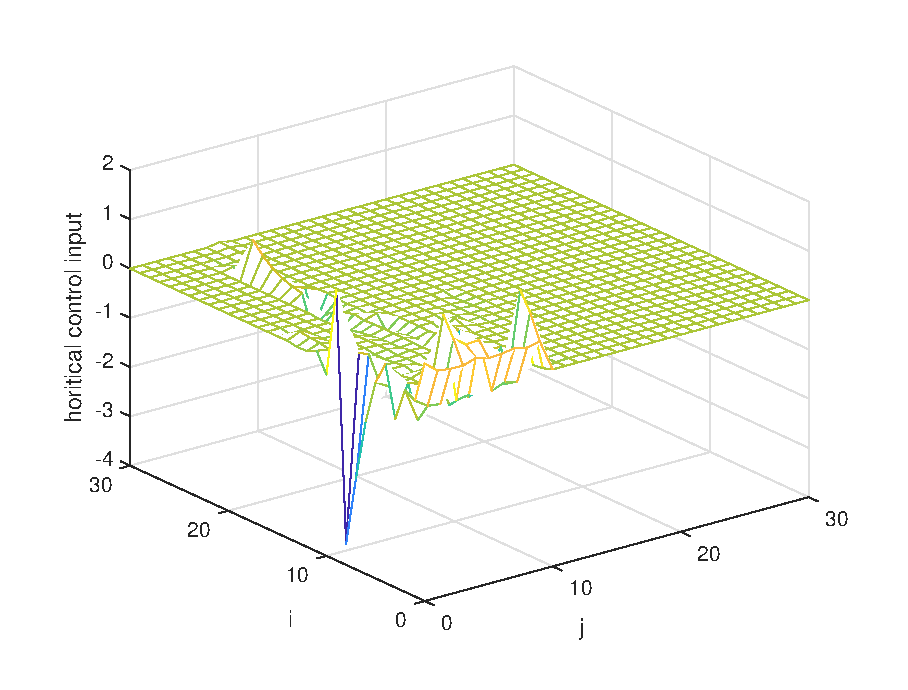
\includegraphics[scale=0.6]{./figures/qc/simulation/hU.eps}\\ 
		\caption{水平控制$u^{v}(i,j)$}
		\label{figqcuh}
	\end{figure}
	
	\begin{figure}[!htb]
		\centering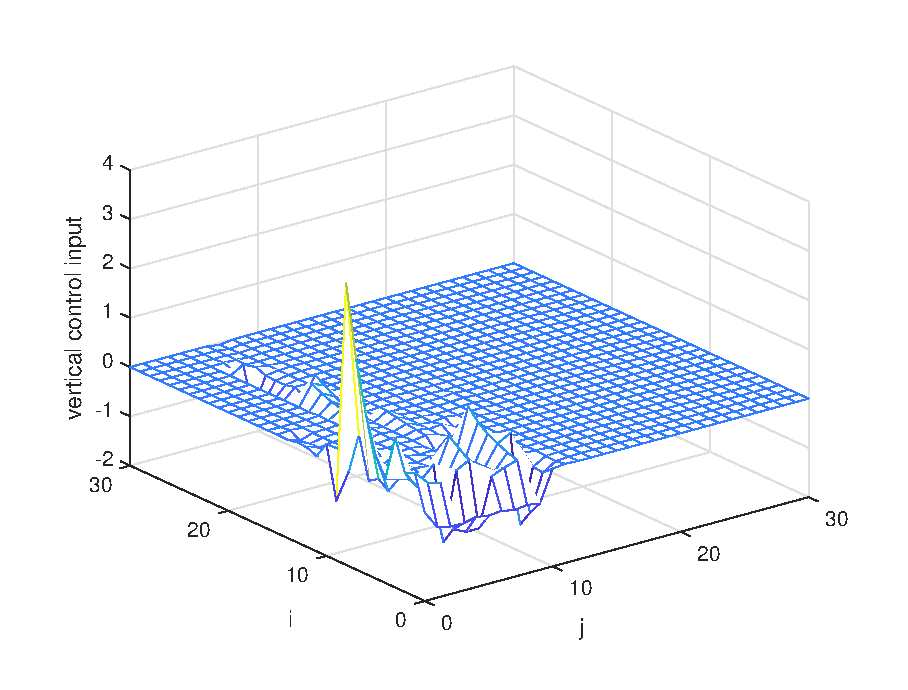
\includegraphics[scale=0.6]{./figures/qc/simulation/vH.eps}\\ 
		\caption{垂直控制$u^{v}(i,j)$}
		\label{figqcuv}
	\end{figure}

\section{小结} \label{conclusion} 	
	本章我们研究了Roesser模型下的二维Markov跳变系统的异步二次型控制问题。考虑到控制器不能获得完整的系统模态信息,存在控制器模态和系统模态不匹配的现象,因此我们基于隐Markov模型设计了异步二次型控制器。借助线性矩阵不等式及李雅普诺夫函数方法,我们对三种不同的初始条件展开了讨论,分别得到了不同情况下的的最优保成本性能。同时,不管初始条件如何,系统都是渐进均方稳定的。
	
	